\section{Designe of Experiment}
\subsection{Wichtige Wörter}
\begin{itemize}
	\item \textbf{Experiment:} Subjekte oder Objekte einer bewusst geschaffene Situation werden beobachtet
	\begin{itemize}
		\item Kausale Zusammenhänge lassen sich besser durch Experimente zeigen (Einflussgrössen frei einstellbar)
	\end{itemize}
	\item \textbf{Erhebung:} Subjekte oder Objekte werden im Rahmen einer existierenden Situation beobachtet
	\begin{itemize}
		\item Meist zu viele Variablen, Interpretation wird schwierig
	\end{itemize}
	\item \textbf{Statistischer Versuchsplanung - DoE:} Planung, sodass Daten mit statistischen Methoden zielführend ausgewertet werden können
	\begin{itemize}
		\item Möglichst wenige Messungen, für möglichst präzise Schätzungen oder möglichst mächtige Tests
	\end{itemize}
	\item Variablen-Screening um wichtige Grössen zu identifizieren (Screening-Experiment), besonders bei vielen Variablen
	\item \textbf{Primäre Variablen od. Prüffaktoren:} Hauptfrage an das Experiment hängt direkt mit diesen Variablen zusammen
	\begin{itemize}
		\item Bei einer Primären Variabel: Zwei möglichst weit auseinanderliegende Einstellungen wählen, und dazwischen gleichmässig verteilte Werte prüfen
		\item Bei mehreren Primären Variablen: Variablen sollten möglichst orthogonal sein zueinander (Keine Korelation zwischen einzelnen Variablen)
	\end{itemize}
	\item \textbf{Sekundär Variablen od. Störfaktoren:} Feststellbarer Einfluss auf das Ergebnis des Experiments, müssen nicht zwingend kontrollierbar sein
	\item \textbf{Blockbildung:} mit \glqq künstlichen \grqq Variablen, z.B. für Batches, Produktions-Lose, etc. 
	\item \textbf{Replikate:} Führen zu höheren Genauigkeit, keine Scheinwiederholungen (Messungen gleich nacheinander $\rightarrow$ Randomisieren)
	\item \textbf{Versuchsplan:} Liste aus Versuchsbedingungen, z.B. Welcher Faktor auf welchen Stufen variiert wird
	\begin{itemize}
		\item Vollständig randomisierter Versuchsplan: Bei einem Faktor mit mehreren Stufen mehrere Messungen pro Stufe (aber immer gleich viele). Abarbeitung in Zufälliger Reihenfolge
		\item Block Design: Neben dem Primären Faktor hat es auch ein sekundärer (Stör-) Faktor mit Einfluss auf die Zielvariabel.  Kommt jede \textbf{Stufe} des ersten Faktors in jedem Block mindestens einmal zur Anwendung: Versuchsplan mit vollständigen Blöcken
		\item \textbf{Faktorielle Versuchspläne:} Versuchsplan mit Stufenkombinationen: bei $k$ Primären Faktoren mit je $L$ Stufen. Werden alle Kombinationen getestet ($L^k$ Messungen) ist das der vollständig faktorielle Versuchsplan
		\begin{itemize}
			\item Wenn keine Wechselwirkungen zwischen den Variablen, können unvollständige Versuchpläne eingesetzt werden. Sind diese immernoch ausgewogen (balanciert) sind das fraktionelle Versuchspläne
			\item Haben die Faktoren im vollständig faktoriellen Versuchsplan nur zwei Stufen, dann ist das ein vollständiger $2^k$-faktorieller Versuchsplan (für jeden Faktor werden zwei Messungen gemacht)
		\end{itemize}
	\end{itemize}
\end{itemize}


\subsection{Faktorielle Designs}
\begin{itemize}
	\item Oftmals auch als Varanz-Analyse bezeichnet
	\item Eine Zielgrösse interessiert uns, die nicht direkt messbar ist, jedoch durch Faktoren beeinflusst wird
	\begin{itemize}
		\item z.B. verschiedene Level, Methoden, etc. Alles sind diskrete und nicht kontinuierliche Werte
		\item Es handelt sich also um Faktorvariablen (so z.B. Level 5\%, Level 10\%, Level 15\% oder Methode 1, Methode 2, etc.)
	\end{itemize}
	\item Kann gut in Notch-Box-Plot dargestellt werden (siehe Abbildung \ref{fig:notchedboxplot}). Ein dieser Plots pro gemessenem Level (z.B. Konzentration 5\%, Konzentration 10\%, etc.) In Y-Achse die zu bestimmende Variabel
\end{itemize}
\begin{figure}[h]
	\centering
	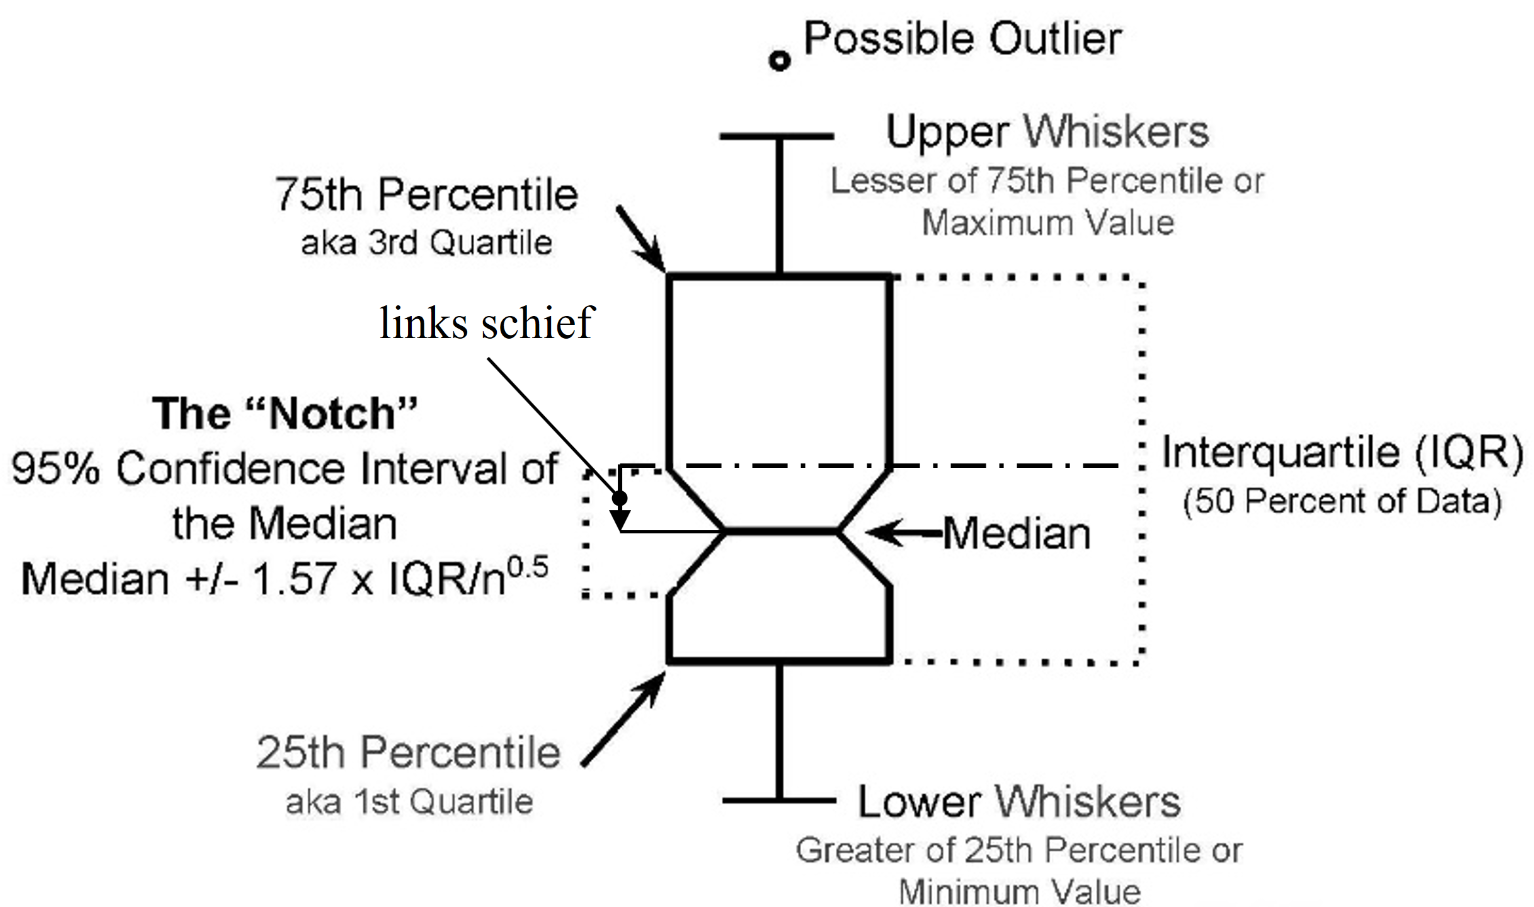
\includegraphics[width=0.5\linewidth]{figures/NotchedBoxPlot}
	\caption{Notch-Boxplot mit Kenngrössen \textit{Quelle:} \cite{C:NotchBoxPlot}}
	\label{fig:notchedboxplot}
\end{figure}

\subsubsection{Anova-Test}
\label{subsubsec:AnovaTest}
\begin{itemize}
	\item Teststatistik die extreme Werte annimmt, wenn sich die Gruppen in er Lage unterscheiden
	\begin{itemize}
		\item Das heisst, wenn der Mittelwert der einzelnen Gruppen auf unterschiedlicher Höhe liegt
		\item In diesem Fall kann die 0-Hypothese verworfen werden (da sich die Ergebnisse einzelner Gruppen signifikant unterscheiden). Es kann somit davon ausgegangen werden, dass die einstellungen der Gruppen das Resultat beeinflussen. 
		\item In Abbildung \ref{fig:Anova} ist gezeigt, wie ein solcher Test aufgebaut ist. Die Ausgabe ist der Quotient zwischen der Streuung zwischen den Gruppen und der Streuung innerhalb der einzelnen Gruppen
		\item Dieser Koeffizient wird als $T$ bezeichnet in der Abbildung ist dieser rot hinterlegt. 
		\item Wenn im R-Output das Signifikanzlevel (Pr($>$F)) klein ist, kann die $H_0$ des F-Tests abgelehnt werden. Mindestens eine der gemessenen Gruppen hat Einfluss. 
	\end{itemize}
	\item Siehe \ref{subsec:RBefehler} für die Anwendung für Wechselwirkungen
\end{itemize}

\begin{figure}[!h]
	\centering
	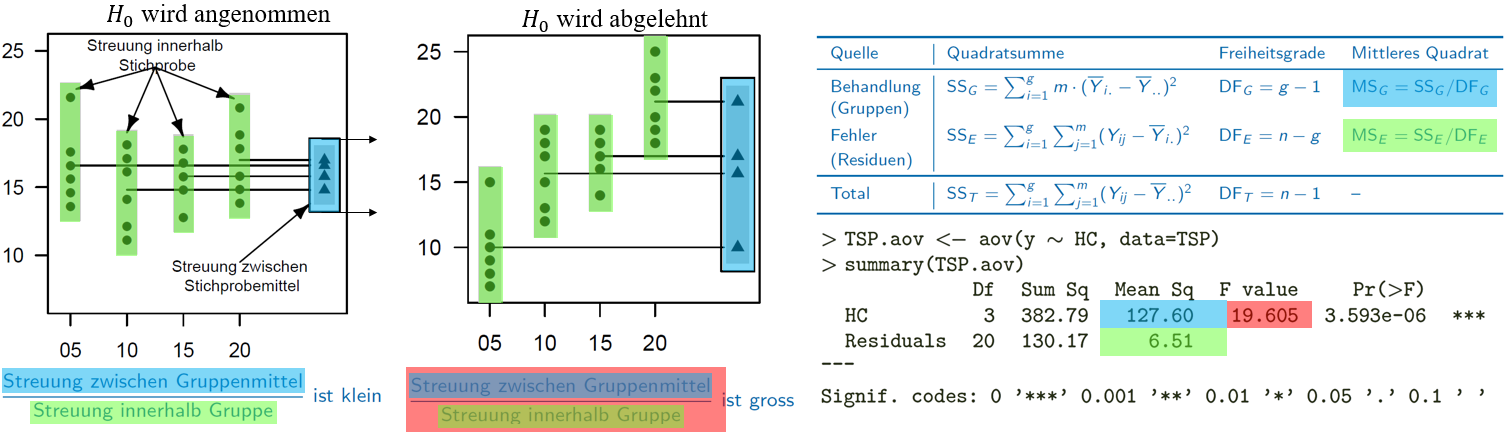
\includegraphics[width=1\linewidth]{./figures/Anova.png}
	\caption{Schema des Anova-Tests. Dieser gibt Auskunft ob $H_0$ über Gruppen abgelehnt oder angenommen wird. \textit{Quelle:}\cite{C:Anova}}
	\label{fig:Anova}
\end{figure}

\subsubsection{Block-Versuchsplan}
\begin{itemize}
	\item Faktor A ist ein primärer Faktor (Behandlungsfaktor)
	\item Faktor B teilt Versuch in Blöcke ein, sekundärer Faktor
	\begin{itemize}
		\item Blöcke sollten möglichst homogen sein, dass Unterschiede innerhalb des Blockes möglichst auf unterschiedliche Behandlungen zurückzuführen ist. 
	\end{itemize}
	\item Man spricht von einem Block-Design
	\item Verlaufen die Linien im Interaction Plot parallel, so kann von Addivität ausgegangen werden
	\begin{itemize}
		\item Y-Achse ist Wechselwirkung zwei verschiedener grössen
		\item X-Achse ist ein Faktor (vorteilhaft ein Primärer Faktor)
	\end{itemize}
\end{itemize}

\textbf{Zwischenstand: bis und mit DoE2}
